% Original experimental-contract schematic, not a model-architecture claim.
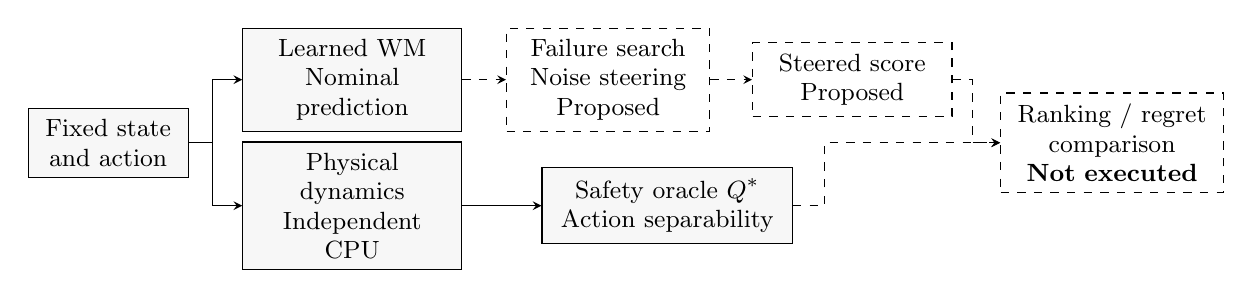
\begin{tikzpicture}[x=1cm,y=1cm,>=stealth,
 box/.style={draw,thin,align=center,inner sep=4pt,minimum height=.85cm,font=\fontsize{9.3}{10.6}\selectfont},
 done/.style={box,fill=black!3},
 proposed/.style={box,dashed,fill=white}]
\node[done,text width=1.75cm] (input) at (.9,.75) {Fixed state\\and action};
\node[done,text width=2.5cm] (wm) at (4,1.55) {Learned WM\\Nominal prediction};
\node[proposed,text width=2.3cm] (steer) at (7.25,1.55) {Failure search\\Noise steering\\Proposed};
\node[proposed,text width=2.25cm] (score) at (10.35,1.55) {Steered score\\Proposed};
\node[done,text width=2.5cm] (physics) at (4,-.05) {Physical dynamics\\Independent CPU};
\node[done,text width=2.9cm] (oracle) at (8,-.05) {Safety oracle $Q^*$\\Action separability};
\node[proposed,text width=2.55cm] (compare) at (13.65,.75) {Ranking / regret\\comparison\\\textbf{Not executed}};
\draw[->] (input.east) -- ++(.3,0) |- (wm.west);
\draw[->] (input.east) -- ++(.3,0) |- (physics.west);
\draw[->,dashed] (wm) -- (steer);
\draw[->,dashed] (steer) -- (score);
\draw[->,dashed] (score.east) -- ++(.25,0) |- (compare.west);
\draw[->] (physics) -- (oracle);
\draw[->,dashed] (oracle.east) -- ++(.4,0) |- (compare.west);
\end{tikzpicture}
